\subsubsection{Testing Suite}\label{subsubsec:testing-suite}
Table \ref{table:testing-suite} below covers what software functions and components of the Nav were verified, how they
were verified, and whether each one passed.
Localization estimates are left untested until integration with the Visual Processing Software Subsystem since they
require both subsystems to work together.
\begin{table}[ht]
    \caption{Navigation Software Subsystem Testing Suite}
    \centering
    \begin{tabular}{P{2cm} P{7cm} P{3.5cm} P{1.5cm}}

        Name & Objectives & Definition & Results \\

        A* & \underline{Correctness} - Is the algorithm implemented in a sound manner? & Unit tests & Pass \\
        Nav & \underline{Safety} - Does it avoid steep (>20° incline) slopes?\linebreak\underline{Adherence to the supplied parameters} - Start and end position and orientation, minimum turn radius\linebreak\underline{Length} - Does it take a reasonable path, not looping or backtracking? & Unit tests & Pass \\
        Mesh to Grid & \underline{Faithfulness} - Does the grid representation closely match the physical terrain? & Human-reviewed & Pass

    \end{tabular}
    \label{table:testing-suite}
\end{table}
\subsubsection{Changes from Previous Verification Plan}\label{subsubsec:changes-to-plan}
Previously, the gradient grid obtained from the triangle mesh did not accurately reflect the physical environment in
some cases.
The biggest issue was that overhangs with vertical faces, when flattened to 2D, appeared as a massive spike in the
terrain heightmap, as if they were solid walls.
\begin{figure}
    \centering
    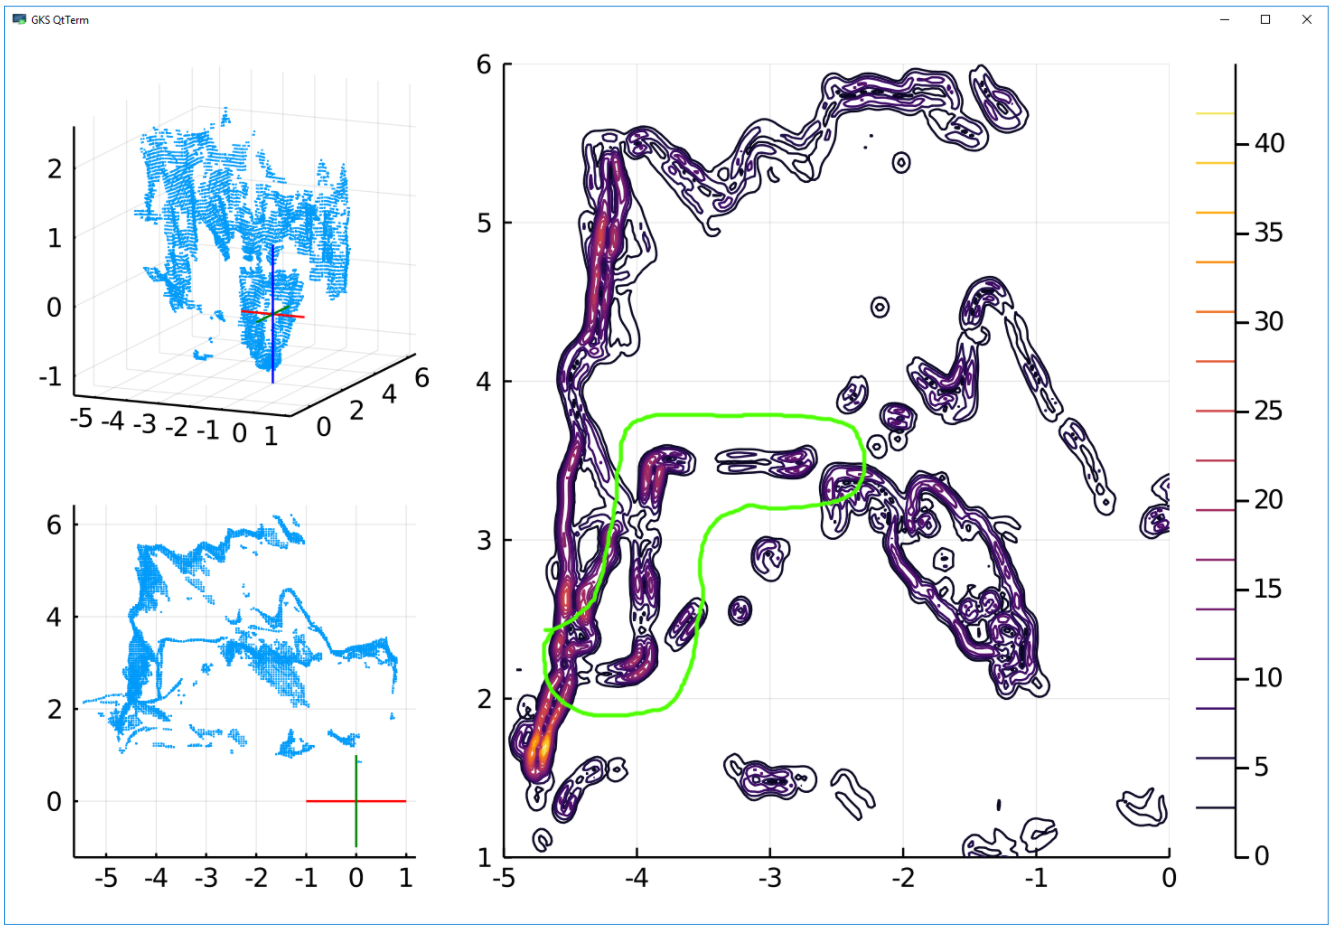
\includegraphics[scale=0.45]{mesh-to-grid-old}
    \caption{
        Visualization of the mesh to gradient grid conversion. The structure circled in green is an overhang with vertical walls that could be passed under, but this mapping would suggest otherwise.\linebreak
        Top-left: Mesh vertices viewed from an oblique angle\linebreak
        Bottom-left: Mesh vertices viewed from above\linebreak
        Right: Contour plot of the gradient magnitude
    }
\end{figure}
This was worked around by ignoring mesh vertices more than 1 meter above the camera's current position.
The 1 meter was chosen arbitrarily to represent the height of the robot; this will eventually be a configurable
parameter.
That way, only overhangs low enough to potentially hit the robot will be treated as a wall.
\begin{figure}
    \centering
    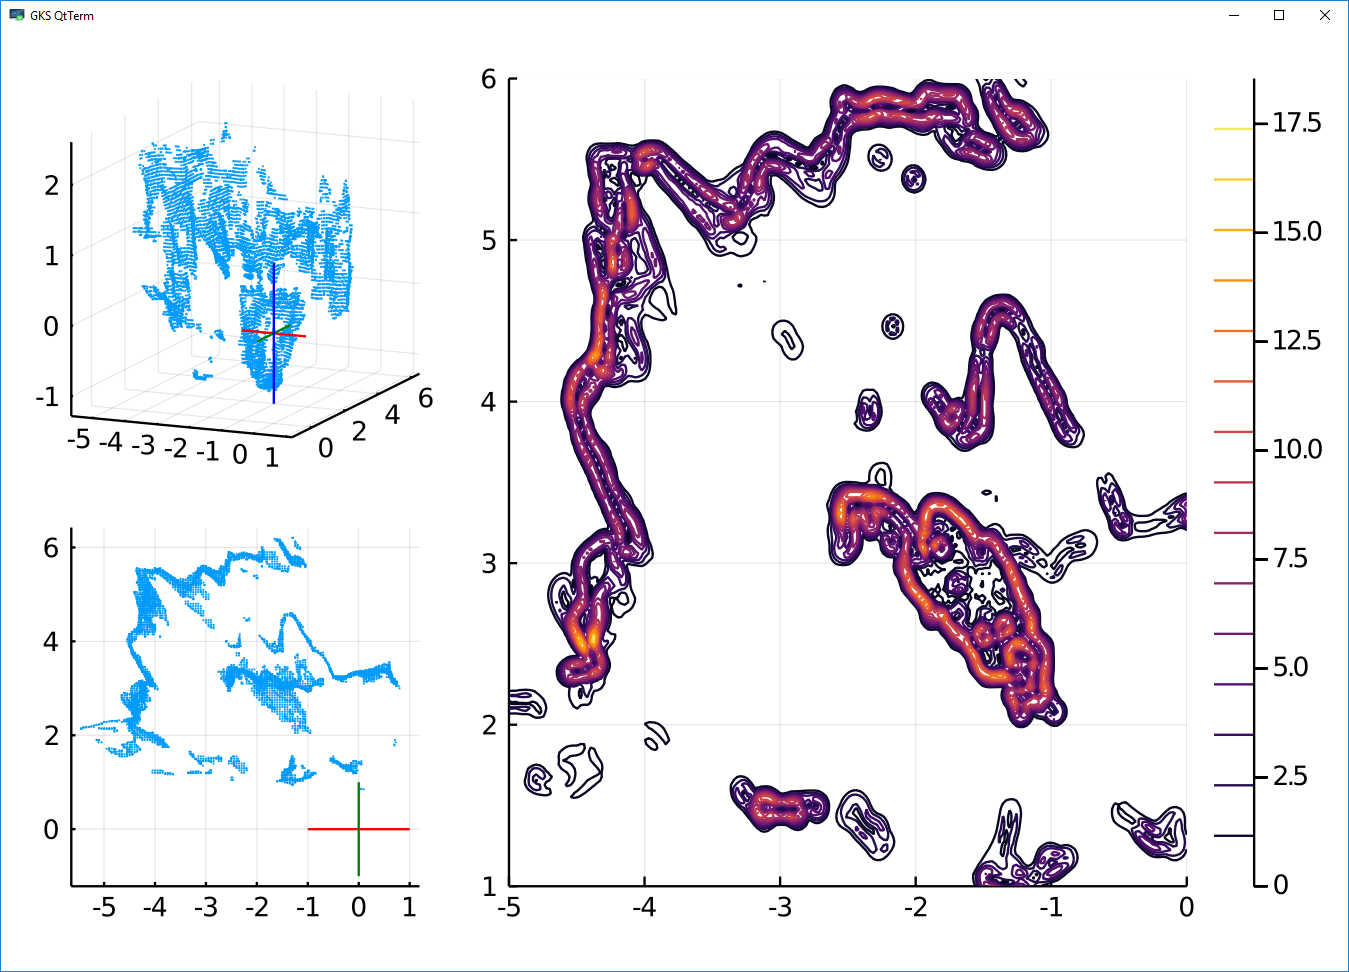
\includegraphics[scale=0.45]{mesh-to-grid}
    \caption{Improved mesh-to-grid.}
\end{figure}